\newpage
\section{Appendix}
%\thispagestyle{empty}
%\pagenumbering{Roman} 	% R XI and r xi
%\addcontentsline{toc}{section}{Appendix}

%%% table settings
\setcounter{table}{0}
\renewcommand{\thetable}{A\arabic{table}}

\setcounter{figure}{0}
\renewcommand{\thefigure}{A\arabic{figure}}

\begin{figure}[!h]
	\caption{Marginal Effects of Left-Right Scale}
	\label{lrscale_probs}
	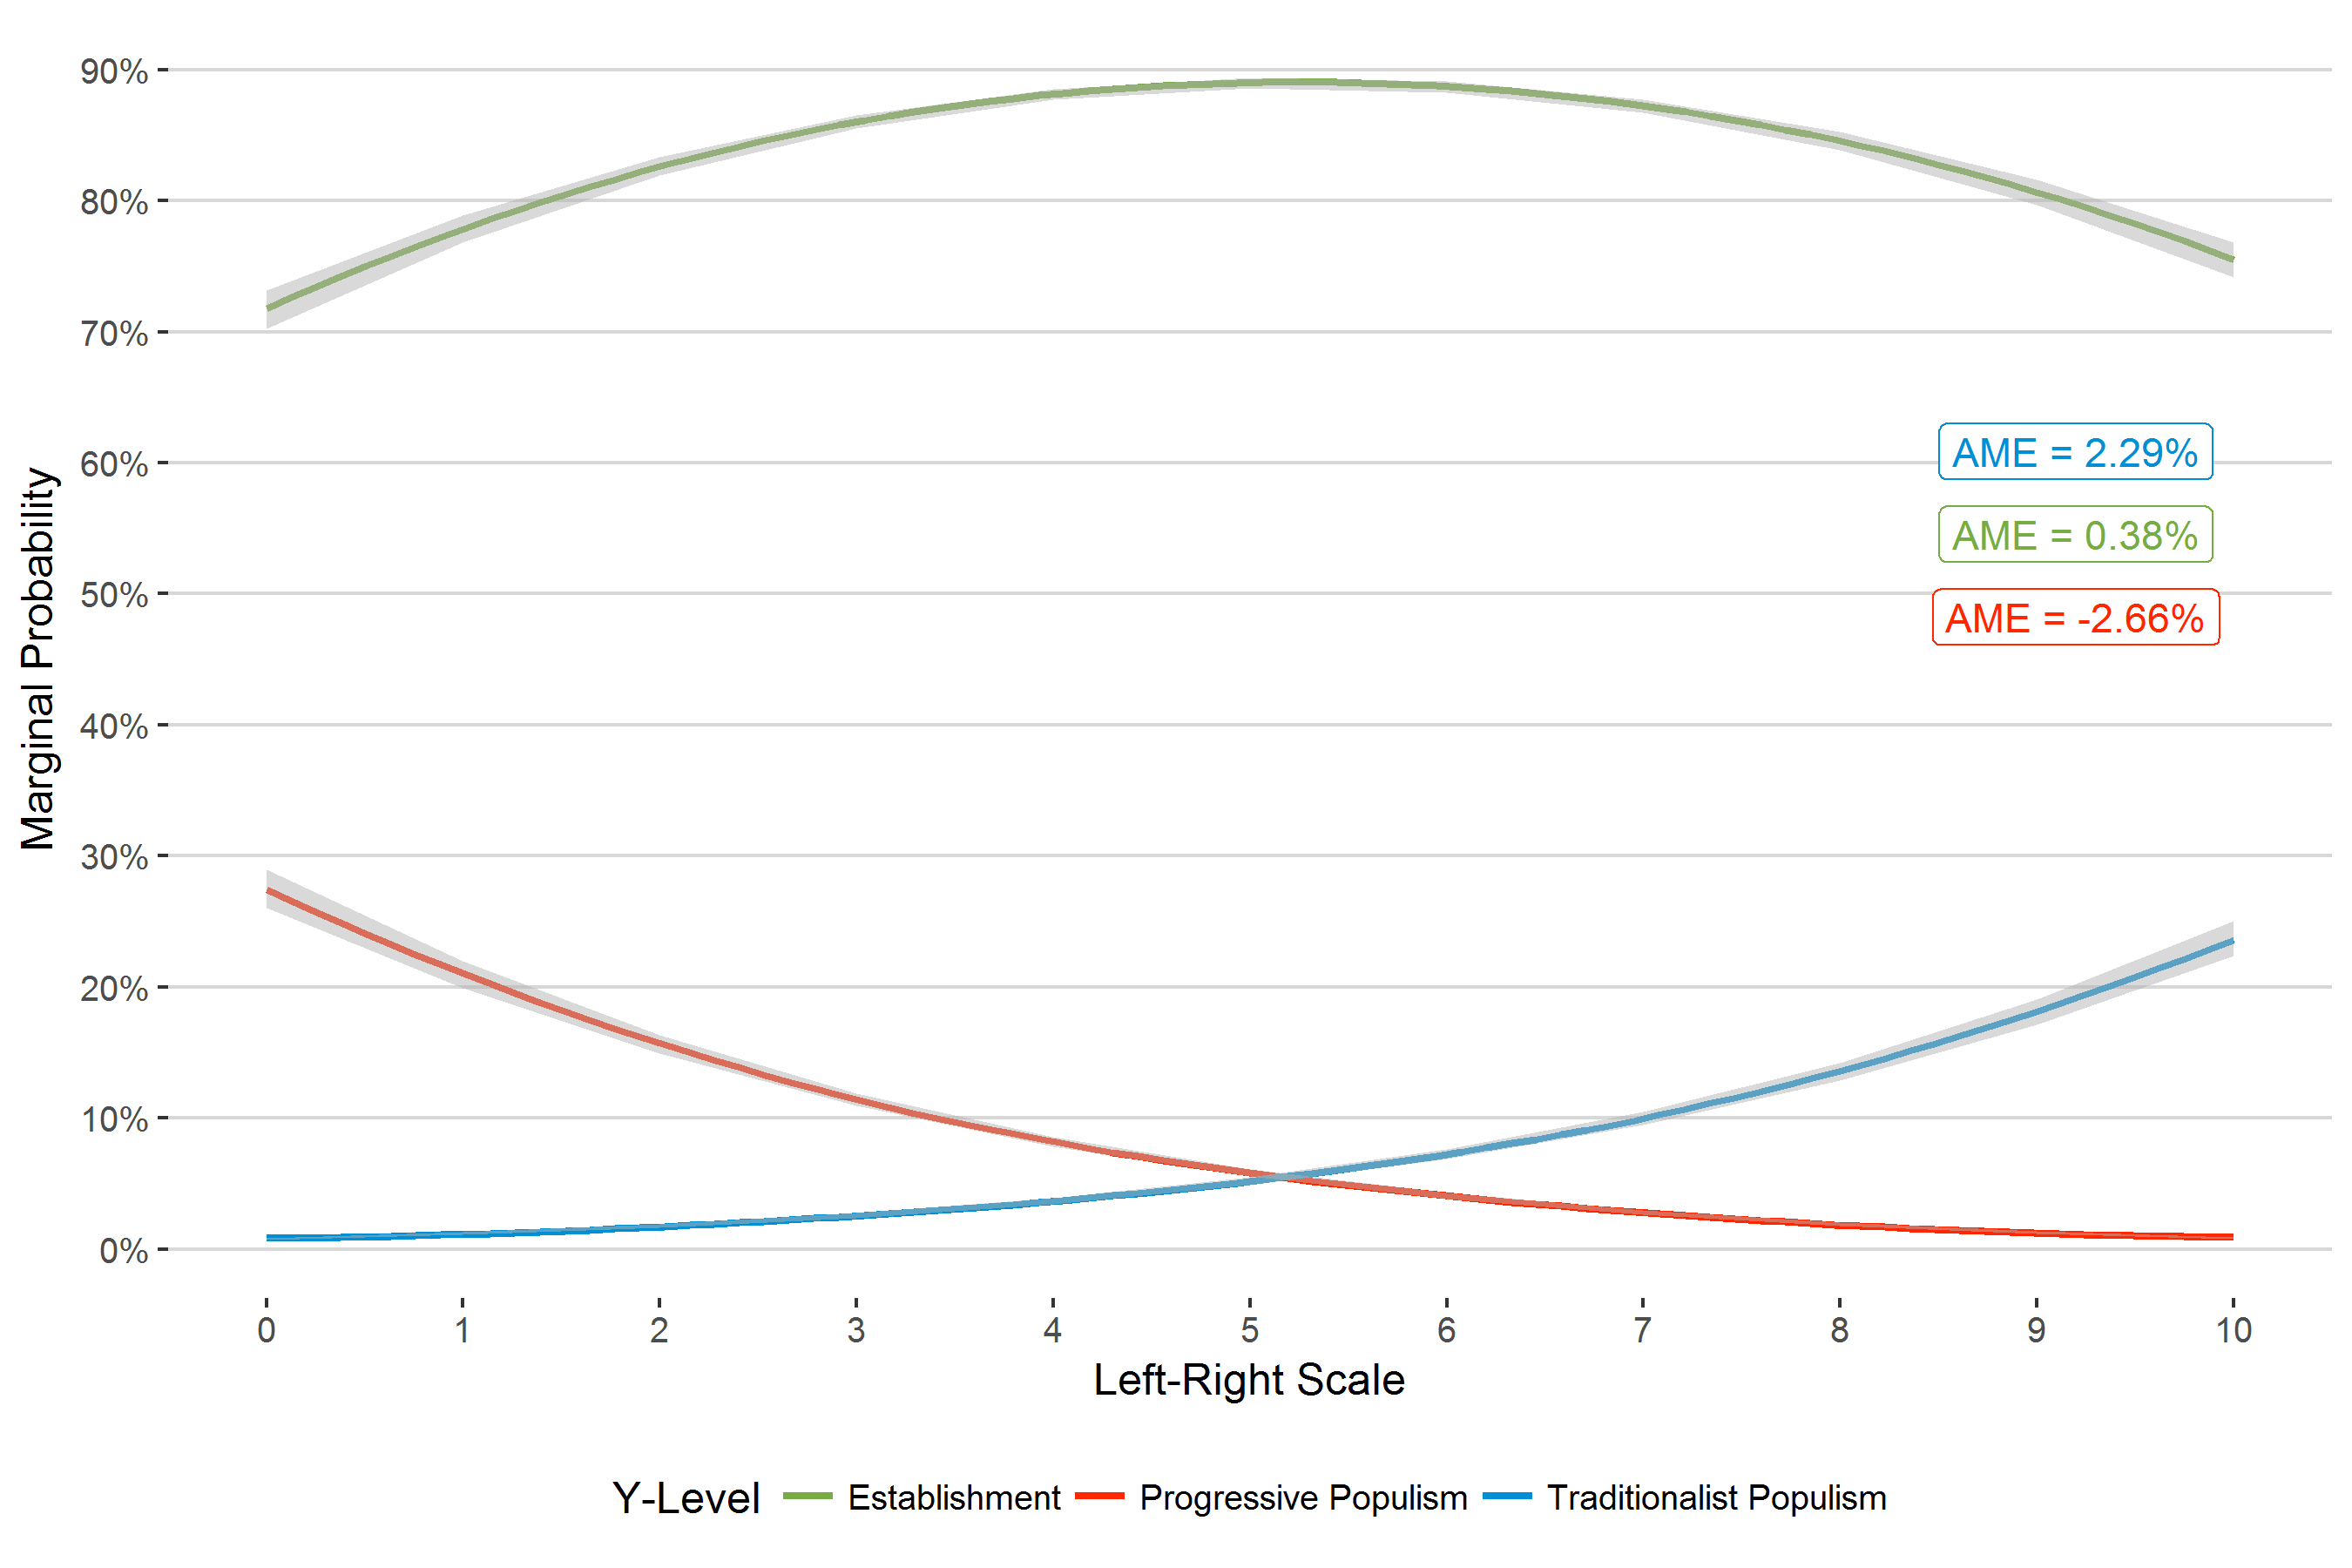
\includegraphics[width=\textwidth]{images/lrscale_probs.png}
	\flushright
	{\scriptsize Based on Model 4. Source: ESS Data Round 5 - 8; N = 68403. \par}
\end{figure}





\small
\begin{landscape}
\begin{longtable}[c]{@{\extracolsep{\fill}}rlllrrl}
		\caption{Party Alignment}
		\label{alignment}\\
		\hline
		& Country & Party Code & Party Name & Populism Score & Prog. - Trad. Score & Type \\ \hline
		\endhead
		%
		\hline
		\endfoot
		%
		\endlastfoot
		%
		\tiny
1 & Austria & aus\_NEOS & Liberal Forum & 35.49 & 19.01 & Establishment \\ 
  2 & Austria & aus\_GRUNE & The Austrian Green Party & 26.27 & 6.11 & Establishment \\ 
  3 & Austria & aus\_SPO & Social Democratic Party of Austria & 17.10 & 32.93 & Establishment \\ 
  4 & Austria & aus\_OVP & Austrian Peoples Party & 7.39 & 63.75 & Establishment \\ 
  5 & Austria & aus\_FPO & Freedom Party of Austria & 82.56 & 89.16 & Traditionalist Populism \\ 
  6 & Austria & aus\_TeamStronach & Team Stronach for Austria & 73.52 & 74.80 & Traditionalist Populism \\ 
  7 & Austria & aus\_BZO & Alliance for the Future of Austria & 69.79 & 70.97 & Traditionalist Populism \\ 
  8 & Belgium & be\_NVA & Peoples Union New Flemish Alliance & 46.54 & 62.08 & Establishment \\ 
  9 & Belgium & be\_FDF & Francophone Democratic Front & 26.05 & 31.90 & Establishment \\ 
  10 & Belgium & be\_Groen & Agalev Green! & 19.16 & 2.23 & Establishment \\ 
  11 & Belgium & be\_ECOLO & Ecolo & 18.73 & 1.66 & Establishment \\ 
  12 & Belgium & be\_PS & Socialist Party & 18.71 & 14.39 & Establishment \\ 
  13 & Belgium & be\_SPA & Socialistische Partij & 18.71 & 13.36 & Establishment \\ 
  14 & Belgium & be\_CDH & Christian Social Party & 12.09 & 35.02 & Establishment \\ 
  15 & Belgium & be\_CD\&V & Christian Peoples Party & 10.39 & 42.25 & Establishment \\ 
  16 & Belgium & be\_MR & Liberal Reformist Party & 9.94 & 34.85 & Establishment \\ 
  17 & Belgium & be\_VLD & Open Flemish Liberals and Democrats & 8.24 & 34.94 & Establishment \\ 
  18 & Belgium & be\_PVDA & Workers Party of Belgium & 71.95 & 12.80 & Progressive Populism \\ 
  19 & Belgium & be\_VB & Flemish Bloc Flemish Interest & 81.97 & 84.58 & Traditionalist Populism \\ 
  20 & Belgium & be\_PP & Peoples Party & 69.40 & 77.95 & Traditionalist Populism \\ 
  21 & Bulgaria & bul\_ABV & Alternative for Bulgarian Revival & 40.97 & 49.17 & Establishment \\ 
  22 & Bulgaria & bul\_BSP & Coalition for Bulgaria & 32.55 & 51.85 & Establishment \\ 
  23 & Bulgaria & bul\_DPS & Movement for Rights and Freedoms & 26.54 & 44.59 & Establishment \\ 
  24 & Bulgaria & bul\_GERB & Citizens for European Development of Bulgaria & 24.78 & 49.49 & Establishment \\ 
  25 & Bulgaria & bul\_DSB & Democrats for a Strong Bulgaria & 24.39 & 36.47 & Establishment \\ 
  26 & Bulgaria & bul\_SDS & United Democratic Forces & 23.89 & 33.89 & Establishment \\ 
  27 & Bulgaria & bul\_DBG & Bulgaria for Citizens Movement & 23.64 & 29.20 & Establishment \\ 
  28 & Bulgaria & bul\_ATAKA & National Union Attack Attack & 93.85 & 95.62 & Traditionalist Populism \\ 
  29 & Bulgaria & bul\_VMRO-BND & Gergiovden-VMRO & 75.29 & 87.17 & Traditionalist Populism \\ 
  30 & Bulgaria & bul\_NFSB & National Front for the Salvation of Bulgaria & 75.22 & 83.07 & Traditionalist Populism \\ 
  31 & Bulgaria & bul\_BBT & Bulgaria without Censorship & 64.59 & 76.52 & Traditionalist Populism \\ 
  32 & Croatia & cro\_HSP-AS & Ante Starcevic & 66.55 & 89.22 & Traditionalist Populism \\ 
  33 & Cyprus & cyp\_EDEK & Movement for Social Democracy EDEK & 41.78 & 44.53 & Establishment \\ 
  34 & Cyprus & cyp\_EVROKO & European Party & 28.91 & 66.13 & Establishment \\ 
  35 & Cyprus & cyp\_DIKO & Democratic Party & 27.79 & 59.19 & Establishment \\ 
  36 & Cyprus & cyp\_DISY & Democratic Rally & 17.17 & 52.97 & Establishment \\ 
  37 & Cyprus & cyp\_AKEL & Progressive Party of Working People & 52.40 & 21.37 & Progressive Populism \\ 
  38 & Cyprus & cyp\_KOP & Ecological and Environmental Movement & 49.27 & 38.98 & Progressive Populism \\ 
  39 & Czech Republic & cz\_ODS & Civic Democratic Party & 42.95 & 55.58 & Establishment \\ 
  40 & Czech Republic & cz\_SZ & Green Party & 31.28 & 6.31 & Establishment \\ 
  41 & Czech Republic & cz\_KDU-CSL & Christian Democratic Union & 13.72 & 74.54 & Establishment \\ 
  42 & Czech Republic & cz\_CSSD & Czech Social Democratic Party & 12.24 & 35.68 & Establishment \\ 
  43 & Czech Republic & cz\_TOP09 & Top09 & 9.41 & 44.34 & Establishment \\ 
  44 & Czech Republic & cz\_SVOBODNI & Party of Free Citizens & 82.00 & 46.09 & Progressive Populism \\ 
  45 & Czech Republic & cz\_ANO2011 & ANO 2011, Action of Dissatisfied Citizens & 53.27 & 39.33 & Progressive Populism \\ 
  46 & Czech Republic & cz\_USVIT & Dawn of Direct Democracy & 87.29 & 83.85 & Traditionalist Populism \\ 
  47 & Czech Republic & cz\_KSCM & Communist Party of Bohemia and Moravia & 63.08 & 61.38 & Traditionalist Populism \\ 
  48 & Denmark & dk\_LA & Liberal Alliance & 40.23 & 28.35 & Establishment \\ 
  49 & Denmark & dk\_SF & Socialist Peoples Party & 31.91 & 18.42 & Establishment \\ 
  50 & Denmark & dk\_KF & Conservative Peoples Party & 22.43 & 64.08 & Establishment \\ 
  51 & Denmark & dk\_V & Venstre, Liberal Party of Denmark & 21.33 & 54.18 & Establishment \\ 
  52 & Denmark & dk\_SD & Social Democrats & 19.79 & 41.05 & Establishment \\ 
  53 & Denmark & dk\_RV & Radical Left-Social Liberal Party & 2.16 & 12.12 & Establishment \\ 
  54 & Denmark & dk\_FolkB & Peoples Movement Against the EU & 89.43 & 9.90 & Progressive Populism \\ 
  55 & Denmark & dk\_EL & Unity List-Red/Green Alliance & 71.98 & 5.96 & Progressive Populism \\ 
  56 & Denmark & dk\_DF & Danish Peoples Party & 76.57 & 79.82 & Traditionalist Populism \\ 
  57 & Estonia & est\_EVE & Estonian Free Party & 48.08 & 46.22 & Establishment \\ 
  58 & Estonia & est\_EER & Estonian Greens & 45.02 & 33.61 & Establishment \\ 
  59 & Estonia & est\_EK & Estonian Center Party & 38.76 & 45.51 & Establishment \\ 
  60 & Estonia & est\_SDE & Social Democratic Party & 14.96 & 21.26 & Establishment \\ 
  61 & Estonia & est\_IRL & Pro Patria and Res Publica Union & 9.23 & 58.42 & Establishment \\ 
  62 & Estonia & est\_ER & Estonian Reform Party & 2.68 & 33.05 & Establishment \\ 
  63 & Finland & fin\_KESK & Finnish Center Party & 37.64 & 61.72 & Establishment \\ 
  64 & Finland & fin\_KD & Finish Christian League Christian Democrats & 34.68 & 79.73 & Establishment \\ 
  65 & Finland & fin\_VIHR & Green League & 28.42 & 2.89 & Establishment \\ 
  66 & Finland & fin\_SDP & Social Democratic Party of Finland & 22.25 & 30.29 & Establishment \\ 
  67 & Finland & fin\_RKP/SFP & Swedish Peoples Party & 7.39 & 20.46 & Establishment \\ 
  68 & Finland & fin\_KOK & National Coalition Party & 4.35 & 50.82 & Establishment \\ 
  69 & Finland & fin\_VAS & Left Alliance & 52.76 & 11.17 & Progressive Populism \\ 
  70 & Finland & fin\_PS & True Finns & 91.15 & 89.52 & Traditionalist Populism \\ 
  71 & France & fr\_EELV & Green Party & 31.73 & 3.73 & Establishment \\ 
  72 & France & fr\_MODEM & Union for French Democracy & 27.98 & 50.58 & Establishment \\ 
  73 & France & fr\_PRG & Left Radical Party & 26.34 & 28.06 & Establishment \\ 
  74 & France & fr\_UMP & Rally for the Republic & 25.72 & 71.27 & Establishment \\ 
  75 & France & fr\_PS & Socialist Party & 23.76 & 27.70 & Establishment \\ 
  76 & France & fr\_PRV & Radical Party & 23.54 & 51.51 & Establishment \\ 
  77 & France & fr\_NC & New Center & 18.55 & 56.16 & Establishment \\ 
  78 & France & fr\_AC & Centrist Alliance & 14.69 & 54.40 & Establishment \\ 
  79 & France & fr\_PG & Left Party & 86.37 & 17.96 & Progressive Populism \\ 
  80 & France & fr\_PCF & French Communist Party & 68.92 & 28.10 & Progressive Populism \\ 
  81 & France & fr\_Ensemble & Together & 68.40 & 32.57 & Progressive Populism \\ 
  82 & France & fr\_FN & National Front & 96.68 & 88.58 & Traditionalist Populism \\ 
  83 & France & fr\_MPF & Rally for France/Movement for France & 84.67 & 89.27 & Traditionalist Populism \\ 
  84 & Germany & ge\_CSU & Christian Social Union in Bavaria & 25.30 & 75.16 & Establishment \\ 
  85 & Germany & ge\_Grunen & Alliance 90 The Greens & 13.53 & 9.87 & Establishment \\ 
  86 & Germany & ge\_FDP & Free Democratic Party & 12.20 & 27.88 & Establishment \\ 
  87 & Germany & ge\_SPD & Social Democratic Party of Germany & 8.46 & 32.99 & Establishment \\ 
  88 & Germany & ge\_CDU & Christian Democratic Union of Germany & 5.78 & 55.92 & Establishment \\ 
  89 & Germany & ge\_DieTier & Human Environment Animal Protection & 75.44 & 9.59 & Progressive Populism \\ 
  90 & Germany & ge\_LINKE & Party of Democratic Socialism & 59.25 & 32.11 & Progressive Populism \\ 
  91 & Germany & ge\_Piraten & Pirate Party of Germany & 52.50 & 7.66 & Progressive Populism \\ 
  92 & Germany & ge\_NPD & German Peoples Union & 90.51 & 97.20 & Traditionalist Populism \\ 
  93 & Germany & ge\_AfD & Alternative for Germany & 83.78 & 85.59 & Traditionalist Populism \\ 
  94 & Greece & gr\_Potami & The River & 33.39 & 14.57 & Establishment \\ 
  95 & Greece & gr\_DIMAR & Democratic Left & 29.91 & 12.96 & Establishment \\ 
  96 & Greece & gr\_PASOK & Panhellenic Socialist Movement & 14.94 & 33.65 & Establishment \\ 
  97 & Greece & gr\_ND & New Democracy & 12.56 & 73.43 & Establishment \\ 
  98 & Greece & gr\_SYRIZA & Coalition of the Left and Progress & 72.41 & 9.22 & Progressive Populism \\ 
  99 & Greece & gr\_XA & Popular AssociationGolden Dawn & 100.00 & 100.00 & Traditionalist Populism \\ 
  100 & Greece & gr\_KKE & Communist Party of Greece & 98.81 & 47.17 & Traditionalist Populism \\ 
  101 & Greece & gr\_ANEL & Independent Greeks & 86.38 & 90.54 & Traditionalist Populism \\ 
  102 & Greece & gr\_LAOS & Popular Orthodox Rally & 76.45 & 88.72 & Traditionalist Populism \\ 
  103 & Hungary & hun\_E14 & Together 2014 & 27.28 & 13.49 & Establishment \\ 
  104 & Hungary & hun\_MSZP & Hungarian Socialist Party & 22.94 & 35.82 & Establishment \\ 
  105 & Hungary & hun\_DK & Democratic Coalition & 22.84 & 18.09 & Establishment \\ 
  106 & Hungary & hun\_LMP & Politics Can Be Different & 50.71 & 16.29 & Progressive Populism \\ 
  107 & Hungary & hun\_JOBBIK & Movement for a Better Hungary & 94.14 & 96.09 & Traditionalist Populism \\ 
  108 & Hungary & hun\_Fidesz & FideszHungarian Civic Union & 57.61 & 82.36 & Traditionalist Populism \\ 
  109 & Ireland & irl\_FF & Soldiers of Destiny & 15.69 & 59.40 & Establishment \\ 
  110 & Ireland & irl\_Lab & Labour & 13.75 & 34.90 & Establishment \\ 
  111 & Ireland & irl\_FG & Family of the Irish & 7.24 & 54.66 & Establishment \\ 
  112 & Ireland & irl\_PBPA & People Before Profit Alliance & 86.29 & 16.85 & Progressive Populism \\ 
  113 & Ireland & irl\_SP & Socialist Party & 84.11 & 19.73 & Progressive Populism \\ 
  114 & Ireland & irl\_SF & We Ourselves & 76.17 & 33.66 & Progressive Populism \\ 
  115 & Ireland & irl\_GP & Green Party & 45.41 & 26.06 & Progressive Populism \\ 
  116 & Italy & it\_FI & Forward Italy & 48.09 & 66.81 & Establishment \\ 
  117 & Italy & it\_SVP & South Tyrolean Peoples Party & 34.43 & 54.63 & Establishment \\ 
  118 & Italy & it\_VdA & Aosta Valley & 31.90 & 48.42 & Establishment \\ 
  119 & Italy & it\_CD & Democratic Centre & 24.35 & 51.56 & Establishment \\ 
  120 & Italy & it\_PD & Democratic Party & 23.52 & 27.39 & Establishment \\ 
  121 & Italy & it\_NCD & New Centre-Right & 18.99 & 68.71 & Establishment \\ 
  122 & Italy & it\_UDC & Christian Democratic Center & 11.59 & 66.68 & Establishment \\ 
  123 & Italy & it\_SC & Civic Choice & 2.84 & 48.44 & Establishment \\ 
  124 & Italy & it\_M5S & Five Star Movement & 97.30 & 30.75 & Progressive Populism \\ 
  125 & Italy & it\_RC & Communist Refoundation Party & 88.86 & 4.25 & Progressive Populism \\ 
  126 & Italy & it\_SEL & Left and Freedom Left Ecology Freedom & 65.55 & 8.23 & Progressive Populism \\ 
  127 & Italy & it\_LN & Northern League & 93.29 & 80.76 & Traditionalist Populism \\ 
  128 & Italy & it\_Fdl & Brothers of Italy & 70.89 & 83.78 & Traditionalist Populism \\ 
  129 & Latvia & lat\_SDPS & Harmony Centre Social Democratic Party Harmony & 59.65 & 52.22 & Establishment \\ 
  130 & Latvia & lat\_LRA & Latvian Association of Regions & 53.61 & 62.04 & Establishment \\ 
  131 & Latvia & lat\_ZZS & Union of Greens and Farmers & 42.78 & 60.56 & Establishment \\ 
  132 & Latvia & lat\_NA & National Alliance All For Latvia! & 34.15 & 71.23 & Establishment \\ 
  133 & Latvia & lat\_V & Unity & 8.02 & 35.17 & Establishment \\ 
  134 & Latvia & lat\_LKS & For Human Rights in United Latvia & 81.82 & 65.94 & Traditionalist Populism \\ 
  135 & Latvia & lat\_NSL & For Latvia from the Heart & 68.18 & 61.62 & Traditionalist Populism \\ 
  136 & Lithuania & lith\_LVZS & Lithuanian Peasant Party & 49.55 & 59.38 & Establishment \\ 
  137 & Lithuania & lith\_DP & Labour Party & 37.18 & 49.96 & Establishment \\ 
  138 & Lithuania & lith\_TS-LKD & Homeland UnionLithuanian Christian Democrats & 10.96 & 66.26 & Establishment \\ 
  139 & Lithuania & lith\_LSDP & Social Democratic Party of Lithuania & 9.50 & 35.22 & Establishment \\ 
  140 & Lithuania & lith\_LRLS & Liberals Movement of the Republic of Lithuania & 8.27 & 20.53 & Establishment \\ 
  141 & Lithuania & lith\_DK & The Way of Courage & 79.87 & 82.04 & Traditionalist Populism \\ 
  142 & Lithuania & lith\_TT & Order and Justice & 68.82 & 80.06 & Traditionalist Populism \\ 
  143 & Lithuania & lith\_LLRA & Electoral Action of Lithuanias Poles & 53.61 & 69.63 & Traditionalist Populism \\ 
  144 & Netherlands & nl\_50PLUS & 50PLUS & 46.09 & 41.44 & Establishment \\ 
  145 & Netherlands & nl\_SGP & Political Reformed Party & 40.30 & 86.13 & Establishment \\ 
  146 & Netherlands & nl\_CU & ChristianUnion & 37.98 & 63.01 & Establishment \\ 
  147 & Netherlands & nl\_VVD & Peoples Party for Freedom and Democracy & 20.91 & 51.44 & Establishment \\ 
  148 & Netherlands & nl\_CDA & Christian Democratic Appeal & 16.29 & 60.29 & Establishment \\ 
  149 & Netherlands & nl\_PvdA & Labour Party & 16.29 & 27.69 & Establishment \\ 
  150 & Netherlands & nl\_GL & GreenLeft & 9.32 & 3.71 & Establishment \\ 
  151 & Netherlands & nl\_D66 & Democrats 66 & 5.47 & 5.07 & Establishment \\ 
  152 & Netherlands & nl\_SP & Socialist Party & 73.19 & 33.40 & Progressive Populism \\ 
  153 & Netherlands & nl\_PvdD & Party for the Animals & 51.03 & 16.94 & Progressive Populism \\ 
  154 & Netherlands & nl\_PVV & Party for Freedom & 97.10 & 74.40 & Traditionalist Populism \\ 
  155 & Poland & pol\_RP & Your Movement (Palikots Movement) & 27.81 & 1.02 & Establishment \\ 
  156 & Poland & pol\_PSL & Polish Peoples Party & 22.20 & 61.39 & Establishment \\ 
  157 & Poland & pol\_SLD & Alliance of Democratic Left & 14.91 & 21.74 & Establishment \\ 
  158 & Poland & pol\_PO & Civic Platform & 7.83 & 38.22 & Establishment \\ 
  159 & Poland & pol\_KNP & Congress of the New Right & 97.60 & 88.89 & Traditionalist Populism \\ 
  160 & Poland & pol\_SP & United Poland & 71.86 & 85.15 & Traditionalist Populism \\ 
  161 & Poland & pol\_PiS & Law and Justice Party & 63.36 & 81.24 & Traditionalist Populism \\ 
  162 & Poland & pol\_PR & Poland Together & 55.76 & 66.40 & Traditionalist Populism \\ 
  163 & Portugal & por\_PS & Socialist Party & 12.30 & 27.73 & Establishment \\ 
  164 & Portugal & por\_PP & Democratic and Social Center Peoples Party & 7.27 & 66.66 & Establishment \\ 
  165 & Portugal & por\_PSD & Democratic Peoples Party & 0.00 & 49.06 & Establishment \\ 
  166 & Portugal & por\_CDU & Democratic Unitarian Coalition & 80.08 & 25.59 & Progressive Populism \\ 
  167 & Portugal & por\_BE & Left Bloc & 69.46 & 1.27 & Progressive Populism \\ 
  168 & Portugal & por\_MPT & Earth Party & 69.81 & 56.61 & Traditionalist Populism \\ 
  169 & Romania & rom\_PC & Romanian Humanist Party Conservative Party & 28.60 & 66.12 & Establishment \\ 
  170 & Romania & rom\_PMP & Peoples Movement Party & 24.04 & 49.10 & Establishment \\ 
  171 & Romania & rom\_UNPR & National Union for the Progress of Romania & 21.47 & 67.94 & Establishment \\ 
  172 & Romania & rom\_UDMR & Hungarian Democratic Union of Romania & 21.04 & 39.52 & Establishment \\ 
  173 & Romania & rom\_PSD & Social Democratic Party & 19.88 & 62.72 & Establishment \\ 
  174 & Romania & rom\_PDL & Democratic Party & 17.28 & 50.94 & Establishment \\ 
  175 & Romania & rom\_PNL & National Liberal Party & 15.59 & 49.34 & Establishment \\ 
  176 & Romania & rom\_PLR & Liberal Reformist Party & 15.30 & 45.83 & Establishment \\ 
  177 & Romania & rom\_PP-DD & Peoples PartyDan Diaconescu & 63.75 & 80.79 & Traditionalist Populism \\ 
  178 & Slovakia & slo\_NOVA & New Majority & 49.06 & 70.48 & Establishment \\ 
  179 & Slovakia & slo\_Siet & Net / Network & 42.58 & 68.67 & Establishment \\ 
  180 & Slovakia & slo\_KDH & Christian Democratic Movement & 33.58 & 83.06 & Establishment \\ 
  181 & Slovakia & slo\_SMK-MKP & Party of the Hungarian Coalition & 25.01 & 58.83 & Establishment \\ 
  182 & Slovakia & slo\_Smer-SD & Direction-Third Way & 23.48 & 63.75 & Establishment \\ 
  183 & Slovakia & slo\_SDKU-DS & Slovak Democratic and Christian Union & 20.12 & 48.50 & Establishment \\ 
  184 & Slovakia & slo\_MH & Bridge & 19.90 & 47.86 & Establishment \\ 
  185 & Slovakia & slo\_SaS & Freedom and Solidarity & 61.77 & 27.91 & Progressive Populism \\ 
  186 & Slovakia & slo\_OLaNO & Ordinary People and Independent Personalities & 75.89 & 75.10 & Traditionalist Populism \\ 
  187 & Slovakia & slo\_SNS & Slovak National Party & 73.91 & 94.27 & Traditionalist Populism \\ 
  188 & Spain & esp\_BNG & Galician Nationalist Bloc & 42.40 & 15.88 & Establishment \\ 
  189 & Spain & esp\_UPyD & Union, Progress, and Democracy & 35.48 & 34.61 & Establishment \\ 
  190 & Spain & esp\_C's & CitizensParty of the Citizenry & 33.09 & 37.62 & Establishment \\ 
  191 & Spain & esp\_ERC & Republican Left of Catalonia & 31.20 & 24.81 & Establishment \\ 
  192 & Spain & esp\_PSOE & Spanish Socialist Workers Party & 14.91 & 18.38 & Establishment \\ 
  193 & Spain & esp\_EA & Basque Solidarity & 13.65 & 43.42 & Establishment \\ 
  194 & Spain & esp\_CiU & Convergence and Unity & 12.40 & 62.01 & Establishment \\ 
  195 & Spain & esp\_CC & Coalicion Canaria & 11.54 & 52.78 & Establishment \\ 
  196 & Spain & esp\_EAJ/PNV & Basque Nationalist Party & 11.18 & 58.91 & Establishment \\ 
  197 & Spain & esp\_PP & Peoples Party & 5.47 & 76.62 & Establishment \\ 
  198 & Spain & esp\_Podemos & We Can & 71.66 & 4.82 & Progressive Populism \\ 
  199 & Spain & esp\_IU & United Left & 46.72 & 8.73 & Progressive Populism \\ 
  200 & Spain & esp\_Amaiur & Amaiur & 44.54 & 19.06 & Progressive Populism \\ 
  201 & Spain & esp\_ICV & Initiative for Catalonia & 42.34 & 6.62 & Progressive Populism \\ 
  202 & Sweden & sv\_MP & Environment PartyThe Greens & 37.49 & 4.42 & Establishment \\ 
  203 & Sweden & sv\_SAP & Workers Party-Social Democrats & 21.39 & 23.29 & Establishment \\ 
  204 & Sweden & sv\_C & Center Party & 20.80 & 23.31 & Establishment \\ 
  205 & Sweden & sv\_KD & Christian-Democrats & 17.22 & 55.09 & Establishment \\ 
  206 & Sweden & sv\_M & Moderate Party & 10.99 & 38.02 & Establishment \\ 
  207 & Sweden & sv\_FP & Liberal Peoples Party & 7.48 & 25.59 & Establishment \\ 
  208 & Sweden & sv\_PIRAT & Pirate Party & 67.47 & 5.40 & Progressive Populism \\ 
  209 & Sweden & sv\_FI & Feminist Initative & 67.17 & 0.00 & Progressive Populism \\ 
  210 & Sweden & sv\_V & Left Party & 66.42 & 3.84 & Progressive Populism \\ 
  211 & Sweden & sv\_SD & Sweden Democrats & 92.69 & 90.43 & Traditionalist Populism \\ 
  212 & United Kingdom & uk\_SNP & Scottish National Party & 41.70 & 28.56 & Establishment \\ 
  213 & United Kingdom & uk\_CONS & Conservative Party & 40.67 & 60.20 & Establishment \\ 
  214 & United Kingdom & uk\_PLAID & Party of Wales & 39.65 & 20.54 & Establishment \\ 
  215 & United Kingdom & uk\_LAB & Labour Party & 29.87 & 28.70 & Establishment \\ 
  216 & United Kingdom & uk\_LibDem & Liberal Democratic Party & 15.68 & 17.35 & Establishment \\ 
  217 & United Kingdom & uk\_GREEN & Green Party & 53.00 & 2.90 & Progressive Populism \\ 
  218 & United Kingdom & uk\_UKIP & United Kingdom Independence Party & 95.90 & 90.17 & Traditionalist Populism \\ \hline
\end{longtable}
\end{landscape}



% \setcounter{table}{1}
% \renewcommand{\thetable}{B\arabic{table}}
% \setcounter{figure}{1}
% \renewcommand{\thefigure}{B\arabic{figure}}


%---------------------------------------------------------------------------%
% Eigenständigkeiterklärung
%---------------------------------------------------------------------------%
\clearpage
\section*{Eigenständigkeitserklärung}
\vspace*{2cm}
\begin{center}
	\begin{minipage}[t]{0.8\textwidth}
		Hiermit versichern wir, dass wir die vorliegende Hausarbeit selbständig und nur mit den angegebenen Hilfsmitteln verfasst haben. Alle Passagen, die wir wörtlich als auch sinngemäß aus der Literatur oder aus anderen Quellen wie z. B. Internetseiten entnommen haben, sind deutlich als Zitat mit Angabe der Quelle kenntlich gemacht.
		
		\vspace*{60mm}
		Stuttgart, 15.04.2018
	\end{minipage}
\end{center}


\end{document}

